\documentclass[11pt]{article}
\usepackage{amsfonts,amsmath}
\usepackage{latexsym}
\usepackage{pgfplots, pgfplotstable}
\setlength{\oddsidemargin}{.0in}
\setlength{\evensidemargin}{.0in}
\setlength{\textwidth}{6.5in}
\setlength{\topmargin}{-0.4in}
\setlength{\textheight}{8.5in}

\makeatletter
\long\def\ifnodedefined#1#2#3{%
    \@ifundefined{pgf@sh@ns@#1}{#3}{#2}%
}

\pgfplotsset{
    discontinuous/.style={
    scatter,
    scatter/@pre marker code/.code={
        \ifnodedefined{marker}{
            \pgfpointdiff{\pgfpointanchor{marker}{center}}%
             {\pgfpoint{0}{0}}%
             \ifdim\pgf@y>0pt
                \tikzset{options/.style={mark=*, fill=white}}
                \draw [densely dashed] (marker-|0,0) -- (0,0);
                \draw plot [mark=*] coordinates {(marker-|0,0)};
             \else
                \tikzset{options/.style={mark=none}}
             \fi
        }{
            \tikzset{options/.style={mark=none}}        
        }
        \coordinate (marker) at (0,0);
        \begin{scope}[options]
    },
    scatter/@post marker code/.code={\end{scope}}
    }
}

\makeatother



\begin{document}
\textbf{Keeyon Ebrahimi}\\
\textbf{N14193968}\\
\textbf{Assignment 5}\\
\\ \\ \\
\textbf{Exercise 9.1:}\\
\\
P(X = -1) = $0.2$\\
P(X = 2 ) = $0.5$\\
P(X = 6 ) = $0.3$ \\
\\
Expected Value = $(-1 * 0.2) + (2 * 0.5) + (6 * 0.3)$ = \textbf{$2.6$} 
\\\\
Mean = (-1 + 2 + 6) / 3 = $2\frac{1}{3}$
\\\\
Variance = {\huge $\frac{(-1 - \frac{1}{3}) ^ 2 + (2 - \frac{1}{3}) ^ 2 + (6 - \frac{1}{3}) ^ 2}{3} = \frac{110}{9}$ }
\\\\
Standard Deviation = {\large $\sqrt{Variace} = \sqrt{\frac{110}{9}} = 3.496 $ }
\newpage

\textbf{Exercise 9.2:}
\\ \\
\begin{enumerate}
\item[(a)] Marginal Distributions
\\
$P(X) = [ (0.12 + 0.08 + 0.10), (0.20 + 0.04 + 0.25), (0.08 + 0.10 + 0.03)]$\\
$P(Y) = [ (0.12 + 0.20 + 0.08), (0.08 + 0.04 + 0.10), (0.10 + 0.25 + 0.03)]$\\
\\
{\Large
\textbf{$P(X) = [0.3, 0.49, 0.21]$}\\
\textbf{$P(Y) = [0.4, 0.22, 0.38]$}\\
}
\\
\begin{center}

  \begin{tabular}{ r || c | c | c || c |}
	 & -1 & 1 & 2 & $P(X)$\\ \hline
	 0 & 0.12 & 0.08 & 0.10 & 0.3 \\ \hline   
    1 & 0.20 & 0.04 & 0.25 & 0.49\\ \hline
    3 & 0.08 & 0.10 & 0.03 & 0.21\\ \hline \hline
	$P(Y)$ & 0.4 & 0.22 & 0.38
  \end{tabular}
\end{center}
\item[(b)] $X$ and $Y$ Independent?  \textbf{Solution: No}
\\ \\
Lets label our original joint distribution as $F$. If we are dealing with something that is independent, we should get $F(X, Y) = P(X) * P(Y)$ for all $(x, y)$ in range, or each cell in the table.  This is because $P(A, B) = P(A) * P(B)$ with independent events. \\

\begin{center}
{\Large \textbf{$F(X, Y)$}}\\ 
  \begin{tabular}{ r || c | c | c || c |}
	 & -1 & 1 & 2 & $P(X)$\\ \hline
	 0 & 0.12 & 0.08 & 0.10 & 0.3 \\ \hline   
    1 & 0.20 & 0.04 & 0.25 & 0.49\\ \hline
    3 & 0.08 & 0.10 & 0.03 & 0.21\\ \hline \hline
	$P(Y)$ & 0.4 & 0.22 & 0.38
  \end{tabular}
\end{center}
\begin{center}
{\Large \textbf{$P(X) * P(Y)$}}\\ 
  \begin{tabular}{ r || c | c | c |}
	 & -1 & 1 & 2 \\ \hline
	 0 & 0.12 & 0.07 & 0.11\\ \hline   
    1 & 0.20 & 0.11 & 0.19 \\ \hline
    3 & 0.08 & 0.05 & 0.08 \\ \hline
    \hline
  \end{tabular}
\end{center}
As we can see, when we multiply the margins, we do not get the same the same as $F(X,Y)$, so because $F(X, Y) \neq P(X) * P(Y)$, we know that they are not Independent.
\item[(c)] Exp(X) and Exp(Y)\\
\\
{\Large Exp(X) = $(0 * 0.3) + (1 * 0.49) + (3 * 0.21) = 1.12$}\\
{\Large Exp(Y) = $(-1 * 0.4) + (1 * 0.22) + (2 * 0.38) = 0.58$}\\
\\
\item[(d)] Distribution of $X + Y$. \\ \\
We must first find all the possible values for $X + Y$.  $X$ can be $[0, 1, 3]$.  $Y$ can be $[-1, 1, 2]$\\
This means that the possible values for $X + Y$ are $[-1, 1, 2, 0, 3, 4, 5]$, thus
\\\\
$P(-1) = 0.12$\\
$P(0) = 0.20$\\
$P(1) = 0.08$ \\
$P(2) = 0.10 + 0.04 + 0.08 = 0.22$\\
$P(3) = 0.25$\\
$P(4) = 0.10$\\
$P(5) = 0.03$\\\
\item[(e)] $P(X | Y = 2)$ and $P(Y | X = 1)$
\\
\begin{itemize}
\item[i. ]\textbf{$P(X | Y = 2)$}
\\ \\
We know that $$P(X | Y = 2) = \frac{P(X , Y = 2)}{P(Y = 2)}$$ 
Now lets compute
$$P(Y = 2) = 0.38$$ \\
\begin{center}
\textbf{This means that}
\end{center}
{\Large
$$P(X = 0 | Y = 2) = \frac{0.1}{0.38} = 0.26315 = 26.32\%$$
$$P(X = 1 | Y = 2) = \frac{0.25}{0.38} = 0.65789 = 65.79\%$$
$$P(X = 3 | Y = 2) = \frac{0.03}{0.38} = 0.07894 = 7.895\%$$
}
\item[ii. ] $P(Y | X = 1)$ \\ \\
  We know that $$P(Y | X = 1) = \frac{P(X = 1, Y)}{P(X = 1)}$$ 
Now lets compute
$$P(X = 1) = 0.49$$\\
\begin{center}
\textbf{This means that} \\
\end{center}
{\Large
$$P(Y = -1 | X = 1) = \frac{0.20}{0.49} = 0.40816 = 40.82\%$$
$$P(Y = 1 | X = 1) = \frac{0.04}{0.49} = 0.08163 = 8.163\%$$
$$P(Y = 2 | X = 1) = \frac{0.25}{0.49} = 0.5102 = 51.02\%$$
}
\end{itemize}
\end{enumerate}
\newpage
\textbf{Exercise 9.3: }\\
Let X be a random variable with values 0, 1, 3, and let Y be a random variable with values -1, 1, 2.  Suppose that P(X=0) = 0.5, P(X=1) = 0.4, and P(X=3) = 0.1, with the following values of $P(Y | X)$

\begin{center}
{\Large \textbf{$P(Y | X)$}}\\ 
  \begin{tabular}{ r || c | c | c |}
	 & -1 & 1 & 2 \\ \hline
	 0 & 0.5 & 0.3 & 0.2\\ \hline   
    1 & 0.2 & 0.7 & 0.1 \\ \hline
    3 & 0.4 & 0.1 & 0.5 \\ \hline
    \hline
  \end{tabular}
\end{center}
\begin{enumerate}
\item[(a)] Joint Distribution of $X, Y$\\ \\
We are given all $P(X)$ and also all $P(Y | X)$.  We must now solve for $P(X, Y)$ for the joint distribution.  We know that $P(X) * P(Y | X) = P(X, Y)$, so we just need to multiply in the correct locations to have the correct values.  This results in \\
\begin{center}
{\Large \textbf{$P(X, Y)$}}\\ 
  \begin{tabular}{ r || c | c | c |}
	 & -1 & 1 & 2 \\ \hline
	 0 & 0.25 & 0.15 & 0.1\\ \hline   
    1 & 0.08 & 0.28 & 0.04 \\ \hline
    3 & 0.04 & 0.01 & 0.05 \\ \hline
    \hline
  \end{tabular}
\end{center}

\item[(b)] Distribution of $Y$
\\
\\
{\Large 
$P(Y = -1) = 0.25 + 0.08 + 0.04 = 0.37 = 37\%$\\
$P(Y = 1) = 0.15 + 0.28 + 0.01 = 0.44 = 44\%$\\
$P(Y = 2) = 0.1 + 0.04 + 0.05 = 0.19 = 19\%$\\
}

\item[(c)] Corresponding table for $P(X|Y)$
\\
$$P(X, Y) = P(X | Y) * P(Y)$$
$$\frac{P(X, Y)}{P(Y)} = P(X | Y)$$
\\ \\
\begin{center}
{\Large \textbf{$P(X, Y)$}}\\ 
  \begin{tabular}{ r || c | c | c |}
	 & -1 & 1 & 2 \\ \hline
	 0 & 0.6757 & 0.341 & 0.5263\\ \hline   
    1 & 0.216 & 0.636 & 0.2105 \\ \hline
    3 & 0.108 & 0.0227 & 0.2623 \\ \hline
    \hline
  \end{tabular}
\end{center}
\item[(d)] Distribution of $X + Y$
\\ \\
We must first find all the possible values for $X + Y$.  $X$ can be $[0, 1, 3]$.  $Y$ can be $[-1, 1, 2]$\\
This means that the possible values for $X + Y$ are $[-1, 1, 2, 0, 3, 4, 5]$, thus
\\\\
$P(-1) = 0.25$\\
$P(0) = 0.08$\\
$P(1) = 0.15$ \\
$P(2) = 0.10 + 0.28 + 0.04 = 0.42$\\
$P(3) = 0.04$\\
$P(4) = 0.01$\\
$P(5) = 0.05$\\\
\item[(e)] Exp($X$), Exp($Y$), Exp($X + Y$).
\begin{enumerate}
\item[(i)] \textbf{Exp($X$) $= 0.7$}
\\
$$Exp(X) = (0 * 0.5) + (1 * 0.4) + (3 * 0.1) = 0.7$$
\item[(ii)] \textbf{Exp($Y$) $= 0.45$}
\\
$$Exp(Y) = (-1 * 0.37) + (1 * 0.44) + (2 * 0.19) = 0.45$$
\item[(iii)] \textbf{Exp($X + Y$) $= 1.15$}
\\
\begin{center}
By Theorem 9.8 from page 260, (Proof on page 261), we know that Exp($X + Y$) = Exp($X$) + Exp($Y$)
\end{center}
\vspace{5mm}
$$Exp(X + Y) = Exp(X) + Exp(Y) = 0.7 + 0.45 = 1.15$$
\end{enumerate}
\end{enumerate}
\newpage
\textbf{Problem 6}
\begin{enumerate}
\item[(a)] What is the value of $a$ (written as "a" in the drawing) 
\\ \\
\textbf{Solution: $a = 9$}
\\ \\
With a probability density function, the area under the function has to go to $1$.  This is because $P(A) + P(\overline{A}) = 1$.  So we must find the complete area under the function before $a$, and then find out how long $a$ must be by finding the difference of 1 and the area under the function before $a$.
\\
\begin{itemize}
\item[(i)] Area under $x < 2.0 = 0$
\item[(ii)] Area under $2.0 \leq x < 4.0 = 0.4$
\begin{center}
The equation of this section is $Y = .2$.   To find the area under this part of the function, we take the integral of this equation and give it a range from $2.0$ to $4.0$.
\end{center}
$$ \int_2^4 0.2\ dx = 4.0(0.2) - 2.0(0.2) = 0.4$$
\item[(iii)] Area under $4.0 \leq x < 6.0 = 0.3$
\begin{center}
We must first find the equation of the line from $4.0 \leq x < 6.0$.  
\end{center}
\begin{enumerate}
\vspace{5mm}
\item[•] Slope $4.0 \leq x < 6.0$ 
$$m = \frac{0.1 - 0.2}{6.0 - 4.0} = -0.05$$
\\
\item[•] Equation Y
$$Y = -0.05(x - 4.0) + 0.2 = -0.05x + 0.4$$
\\
\item[•] Area Under Y from $4.0 \leq x < 6.0$
{\Large $$ \int_4^6 -0.05x + 0.4 = (\frac{-0.05}{2}*6^2 + (0.4*6)) - (\frac{-0.05}{2}*4^2 + (0.4*4)) = 0.3$$ }
\end{enumerate}
\item[(iv)]Area under $6.0 \leq a = 0.3$
\\ \\So far our current area under the curve up until $x = 6.0$ is $0.4 + 0.3 = 0.7$ We need total  area under the curve to be $1$, so the remaining amount we need to have under the curve is $1 - 0.7 = 0.3$.\\ \\
\item[(v)] Value of $a = 9$
\\ \\
We need $0.3$ more under the curve, and we know that past $6$, we keep the constant rate of $0.1$. so $$a = 6 + \frac{0.3}{0.1} = 9$$

\end{itemize}
\item[(b)] Using the given $f$, what is the probability that a randomly chosen real number will fall in the interval [5.0, 7.0]?
\\ \\
\textbf{Solution = $0.225 = 22.5\%$}
\\ \\
From $5.0$ to $6.0$, we have a different probability than from $6.0$ to $7.0$.  We need to find the probability through both these intervals and add them together.  
\begin{itemize}
\item[(i)]  Probability from $5.0$ to $6.0 = 0.125$
\\
\begin{center}
As discovered in $Part a. iii$ from this problem, we know that from $5.0$ to $6.0$ we do 
\end{center}
{\Large $$ \int_5^6 -0.05x + 0.4 = (\frac{-0.05}{2}*6^2 + (0.4*6)) - (\frac{-0.05}{2}*5^2 + (0.5*4)) = 0.125$$ }
\item[(ii)] Probability from $6.0$ to $7.0 = 0.1$
\\
$$Value = 0.1 * (7.0 - 6.0) = 0.1$$
\item[(iii)] Probability from $5.0$ to $7.0 = 0.225$
$$Value = 0.125 + 0.1 = 0.225$$
\end{itemize}
\item[(c)] What is the cumulative distribution function? Please both define it as done in the bulleted list above above and produce a drawing.
\\
\begin{itemize}
\item[(i)] Definition
\\
Area from $0$ to $2 = 0$\\ 
Area from $2$ to $4 = 0.4$\\
Area from $4$ to $5 = .175$.  We just apply equation from $Part B i$ but change the integral range to $4$ and $5$ to get this value\\
Area from $5$ to $6 = .125$\\
Area From $6$ to $9 = 0.3$\\
\\ \\
Know these values, we can easily represent the cumulative distribution function\\
\begin{center}
{\Large \textbf{Cumulative Distribution Function}}\\
\vspace{5mm}
  \begin{tabular}{| c | c |}
	 \hline
	 $x$ & $P[ X \leq x]$ \\ \hline
	 0 & $0$ \\ \hline   
	 1 & $0$ \\ \hline   
	 2 & $0$ \\ \hline
	 3 & $0.2$ \\ \hline
	 4 & $0.4$ \\ \hline
	 5 & $0.575$ \\ \hline
	 6 & $0.7$ \\ \hline
	 7 & $0.8$ \\ \hline
	 8 & $0.9$ \\ \hline
	 9 & $1.0$ \\ \hline
  \end{tabular}
\end{center}
\begin{align*}
P(X\leq2) &= 0\\
P(X\leq3) &= 0 + 0.2 = 0.2\\
P(X\leq4) &= 0 + 0.2 + 0.2 = 0.4\\
P(X\leq5) &= 0 + 0.2 + 0.2 + 0.175 = 0.575\\
P(X\leq6) &= 0 + 0.2 + 0.2 + 0.175 + 0.125 = 0.7\\
P(X\leq7) &= 0 + 0.2 + 0.2 + 0.175 + 0.125 + 0.1 = 0.8\\
P(X\leq8) &= 0 + 0.2 + 0.2 + 0.175 + 0.125 + 0.1 + 0.1 = 0.9\\
P(X\leq9) &= 0 + 0.2 + 0.2 + 0.175 + 0.125 + 0.1 + 0.1 + 0.1 = 1.0
\end{align*}

\item[(ii)]Drawing
\\
{\centering
\begin{tikzpicture}
\begin{axis}[
    clip=false,
    jump mark left,
    ymin=0,ymax=1,
    xmin=0, xmax=10,
    every axis plot/.style={very thick},
    discontinuous,
    table/create on use/cumulative distribution/.style={
        create col/expr={\pgfmathaccuma + \thisrow{f(x)}}   
    }
]
\addplot [red] table [y=cumulative distribution]{
x f(x)
0 0
1 0
2 0
3 0.2
4 0.2
5 0.175
6 0.125
7 0.1
8 0.1
9 0.1
};
\end{axis}
\end{tikzpicture}
\par}
\end{itemize}
\end{enumerate}
\end{document}